\chapter{MultiProcess Image Processing Bench}
\begin{figure}[H]
	\centering
	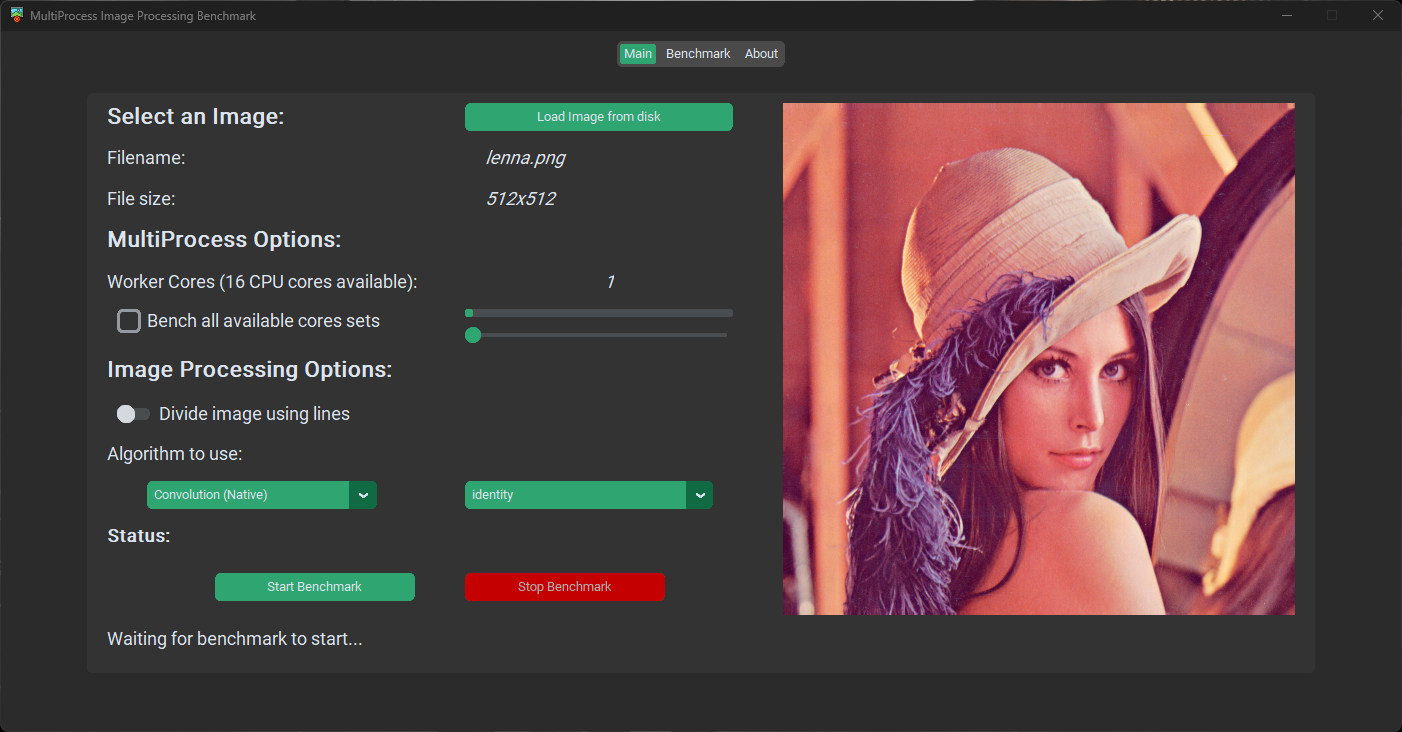
\includegraphics[width=\linewidth]{main-window}
	\caption{Schermata principale dell'applicativo}
\end{figure}
L'applicativo software sviluppato è denominato \textit{"MultiProcess Image Processing Bench"}, a cui, per semplicità, sarà fatto riferimento tramite l'abbreviazione \textit{"Benchmarker"}.\\
\newline
\textit{Benchmarker} è un programma dotato di interfaccia grafica sviluppato in Python 3 con Tkinter, e quindi supportato su MacOS, Linux e Windows. L'applicativo prende in input un'immagine di dimensioni quadrate, ridimensionandola se necessario, esegue un algoritmo di image processing secondo una configurazione utente e restituisce i tempi di esecuzione sotto forma di grafico a barre laterali.\par
Lo scopo di \textit{Benchmarker} è rendere facile ed automatico il confronto delle prestazioni di un certo algoritmo di image processing eseguito su diverse configurazioni di parallelismo.

\section{Uso del programma}
Benchmarker fa uso di librerie esterne, come ad esempio \textit{pillow} e \textit{matplotlib}. Per questo motivo, prima di poter utilizzare il programma è necessario installare tramite \textit{"pip"}, il package installer di Python, le dipendenze in uno dei seguenti modi:
\begin{itemize}
	\item \textit{Global Package}: installare le dipendenze direttamente nel sistema, diventando di fatto globali e accessibili da qualunque script Python eseguito nel sistema;
	\item \textit{Virtual Environment}: creare un ambiente virtuale in cui installare le dipendenze;
\end{itemize}
Una volta installate le dipendenze, per utilizzare Benchmarker, e quindi visualizzare l'interfaccia grafica, è necessario avviare lo script \textit{main.py}.

Una volta aperto il programma è possibile:
\begin{enumerate}
	\item caricare l'immagine su cui eseguire gli algoritmi, qualora l'immagine non fosse di \textit{dimensioni quadrate} verrà chiesto di ridimensionarla;
	\item scegliere il \textit{quantitativo di core} da utilizzare per l'\textit{esecuzione parallela}, il \textit{numero totale di core} dipende dal processore del calcolatore in cui si sta eseguendo l'applicativo;
	\item selezionare la \textit{modalità di suddivisione} in \textbf{linee o quadrati} dell'immagine originale, qualora si scelga la suddivisione in quadrati, il quantitativo di core dovrà essere un \textit{quadrato perfetto};
	\item scegliere se provare o meno tutte le possibili configurazioni parallelo eseguibili nel calcolatore;
	\item selezionare la \textit{tipologia di algoritmo}, ed eventualmente l'algoritmo specifico, inserendo, se richiesti, i parametri dello stesso;
	\item \textit{avviare il benchmark};
\end{enumerate}	
\noindent
Una volta avviato il benchmark, verrà prima eseguita un'\textit{esecuzione sequenziale} dell'algoritmo e successivamente la/le \textit{configurazioni parallele} scelte dall'utente. I risultati verranno visualizzati nell'apposita finestra.
 \begin{figure}[H]
 	\centering
 	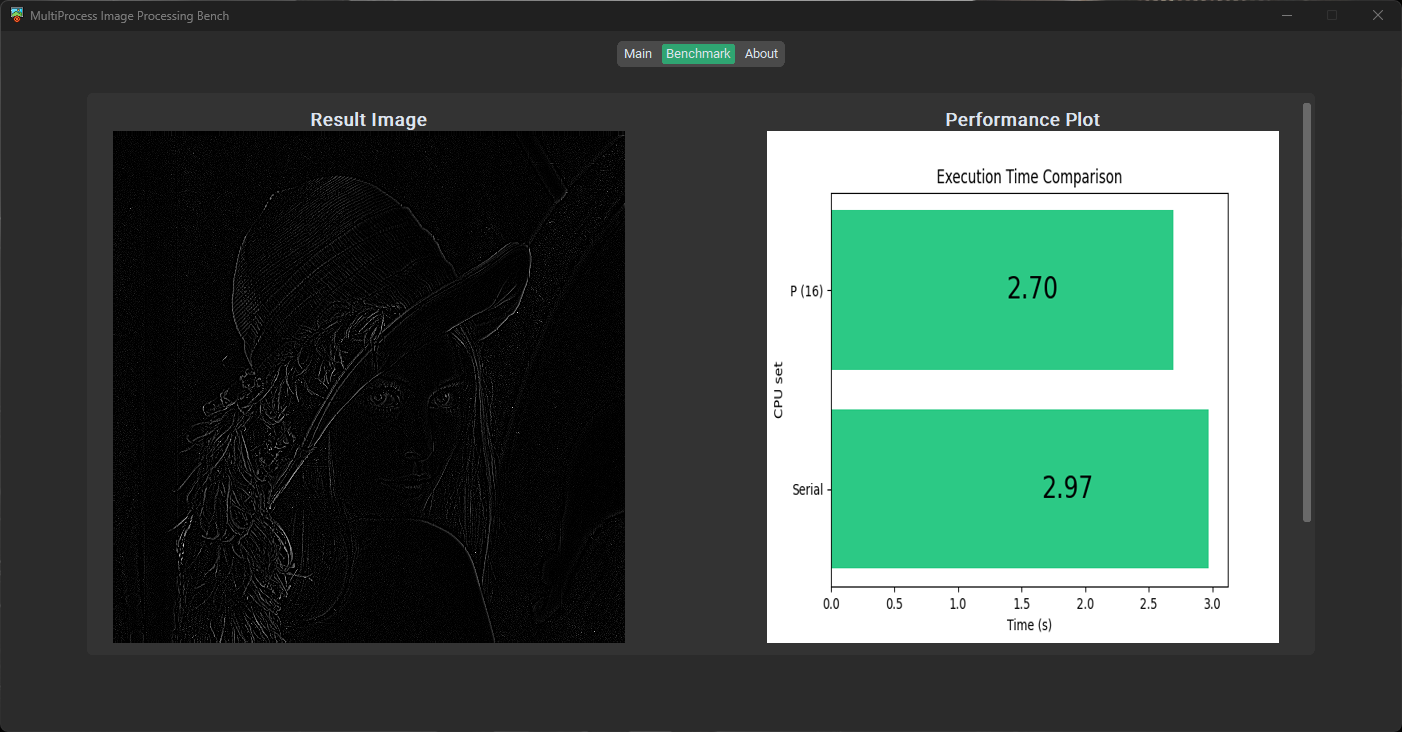
\includegraphics[width=\linewidth]{bench-results}
 	\caption{Esempio di risultati del benchmark}
 \end{figure}

\section{Suddivisione dell'immagine}
Alla base del parallelismo vi è il concetto di \textit{suddividere un grande problema in sotto problemi più piccoli della stessa natura}.
Per quanto riguarda l'image processing tale concetto viene applicato suddividendo un'immagine in \textit{sotto immagini}, ovvero immagini che se riunite ricostruiscono l'immagine originale.
Per tale operazione Benchmarker mette a disposizione due modalità:
\begin{itemize}
	\item \textit{Suddivisione in strisce, o linee}: l'immagine originale viene suddivide in $N$ linee quanti sono i core selezionati per l'esecuzione parallela, ogni processo parallelo eseguirà l'algoritmo sull'immagine parziale assegnatogli e restituirà il risultato parziale, che verrà unito agli altri per formare il risultato completo;
	\begin{itemize}
		\item la \textit{lunghezza della striscia} viene calcolata semplicemente dividendo il lato del quadrato per $N$, numero di linee;
	\end{itemize}
	\item \textit{Suddivisione in quadrati}: l'immagine originale viene suddivide in $M = \sqrt{N}$ quadrati, dove $N$ è il numero di core selezionati per l'esecuzione parallela, ogni processo parallelo eseguirà l'algoritmo sull'immagine parziale assegnatogli e restituirà il risultato parziale, che verrà unito agli altri per formare il risultato completo;
	\begin{itemize}
		\item la \textit{lunghezza del quadrato} viene calcolata semplicemente dividendo il lato del quadrato per $M$, numero di quadrati;
		\item il \textit{numero di core} selezionato per l'esecuzione parallela deve essere un \textit{quadrato perfetto};
	\end{itemize}
\end{itemize}
\noindent La logica per la suddivisione implementata in Python è presente in appendice: \ref{appendix:lines_subdivision}.
 \begin{figure}[H]
	\centering
	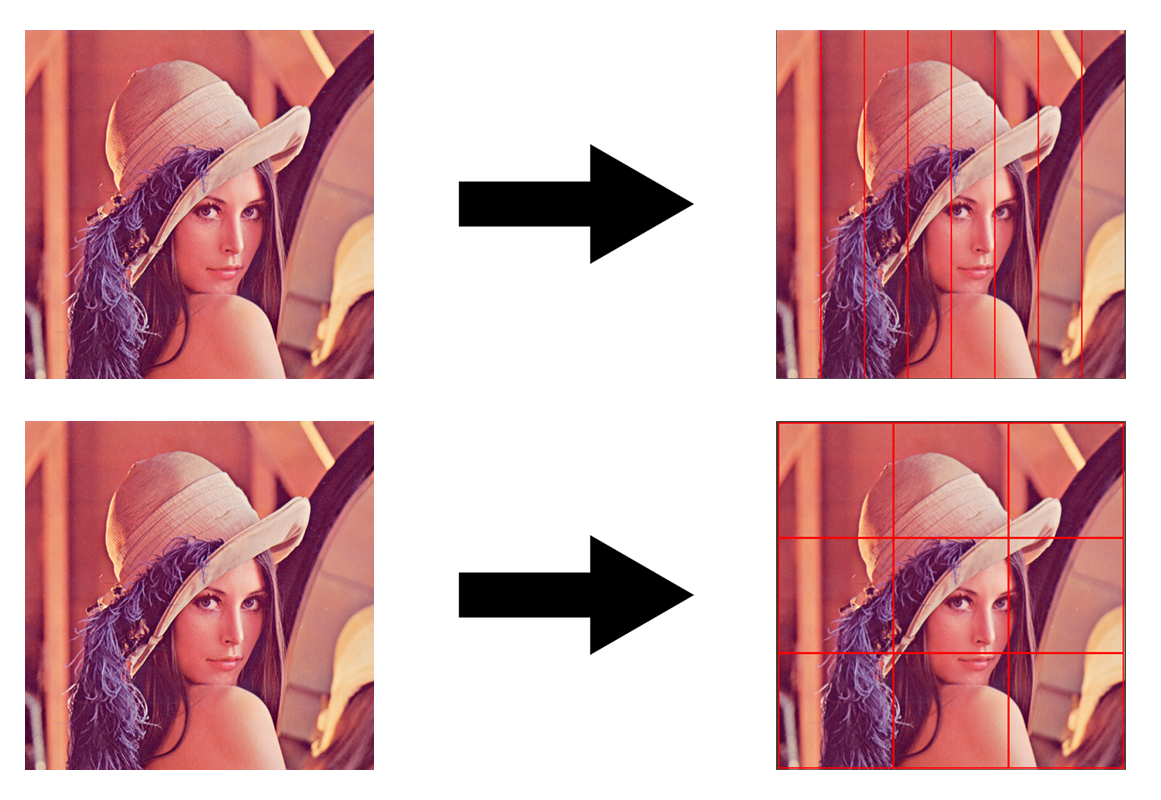
\includegraphics[width=\linewidth]{sub-images-preview}
	\caption{Esempio di suddivisione}
\end{figure}

\section{Algoritmi implementati}
All'interno di Benchmarker sono stati implementati alcuni dei più famosi algoritmi dell'image processing.

Per \textit{scelta di stile e coerenza dei risultati}, tali algoritmi, come convoluzione e operatori morfologici, sono \textit{implementati facendo uso delle funzionalità native di Python} senza l'utilizzo delle funzioni avanzate offerte dalle librerie, in quanto implementate con un riguardo alle prestazioni in C.
\newpage

\subsection{Convoluzione}
La \textit{convoluzione} è un'operazione fondamentale nell'elaborazione delle immagini utilizzata per analizzare e modificare le caratteristiche di un'immagine. In sintesi, la convoluzione consiste nel sovrapporre un \textit{kernel} su un'immagine e calcolare la somma dei prodotti degli elementi sovrapposti del kernel e dei pixel corrispondenti dell'immagine.

Il \textit{kernel} è una piccola matrice di valori numerici, di \textit{dimensioni generalmente dispari}, che definisce come combinare i pixel circostanti durante l'operazione di convoluzione. Ogni elemento del kernel viene moltiplicato con il valore corrispondente del pixel nell'immagine, e i risultati vengono sommati per ottenere il valore convoluto per il pixel centrale.

Questo processo viene ripetuto per ogni pixel dell'immagine.

 \begin{figure}[H]
	\centering
	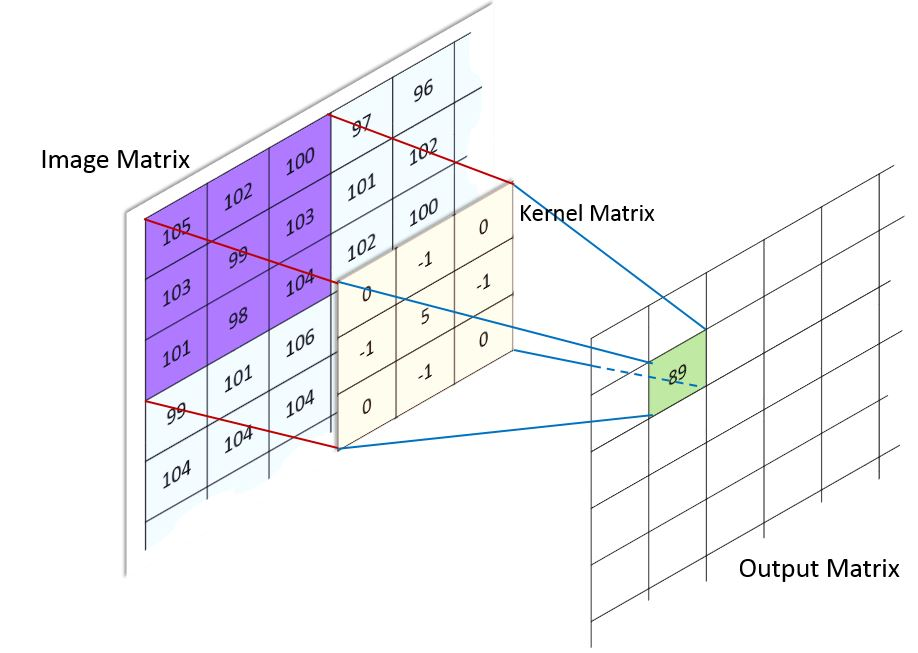
\includegraphics[scale=0.5]{conv-matrix}
	\caption{Schema della convoluzione}
\end{figure}

\noindent La convoluzione viene spesso utilizzata per applicare filtri e operazioni di modifica dell'immagine che richiedono kernel specifici, ideati per ottenere un determinato effetto.

La logica della convoluzione implementata in Python è presente in appendice: \ref{appendix:convolution}

\subsubsection{Identity}
Il kernel \textit{Identity} rappresenta il più semplice filtro convolutivo: non effettua alcuna modifica all'immagine di input.\newline
\begin{equation*}
	\text {Identity Kernel} = 
	\begin{bmatrix}
		0 & 0 & 0 \\
		0 & 1 & 0 \\
		0 & 0 & 0
	\end{bmatrix}
\end{equation*}
\newline Quando viene applicato a un'immagine tramite la convoluzione, mantiene inalterati i valori dei pixel. Ciò significa che il pixel di output nella posizione corrispondente al pixel di input sarà uguale al valore del pixel di input stesso. In pratica, l'immagine convoluta con il kernel identità sarà identica all'immagine di input.
 \begin{figure}[H]
	\centering
	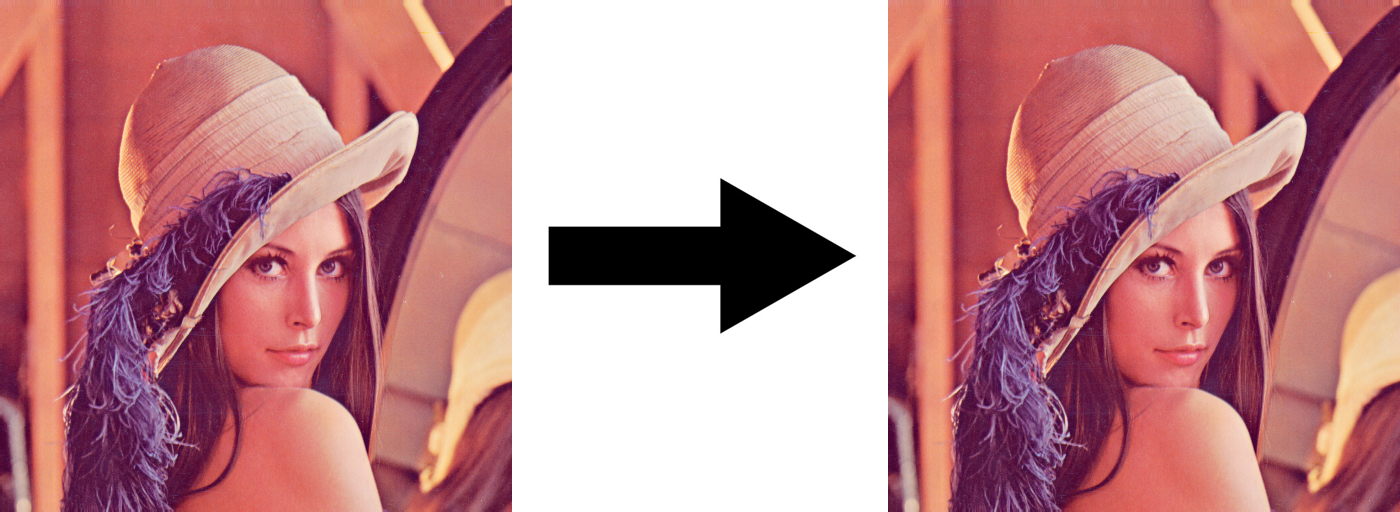
\includegraphics[width=\linewidth]{identity}
	\caption{Esempio di Kernel Identity}
\end{figure}
\subsubsection{Sobel-X e Sobel-Y}
I kernel di \textit{Sobel-X} e \textit{Sobel-Y} sono utilizzati per il rilevamento dei bordi. In particolare, \textit{Sobel-X} evidenzia i cambiamenti di intensità orizzontali, mentre \textit{Sobel-Y} quelli verticali.\newline
\begin{equation*}
	\text {Sobel-X} = 
	\begin{bmatrix}
		-1 & 0 & 1 \\
		-2 & 1 & 2 \\
		-1 & 0 & 1
	\end{bmatrix},
	\quad
	\text {Sobel-Y} = 
	\begin{bmatrix}
		-1 & -2 & -1 \\
		0 & 0 & 0 \\
		1 & 2 & 1
	\end{bmatrix},
\end{equation*}
\newline Quando vengono applicati a un'immagine tramite la convoluzione, calcolano le derivate parziali rispetto alle direzioni orizzontali e verticali, rispettivamente. Questo significa rilevano le variazioni di intensità lungo le linee orizzontali e verticali dell'immagine.
\begin{figure}[H]
	\centering
	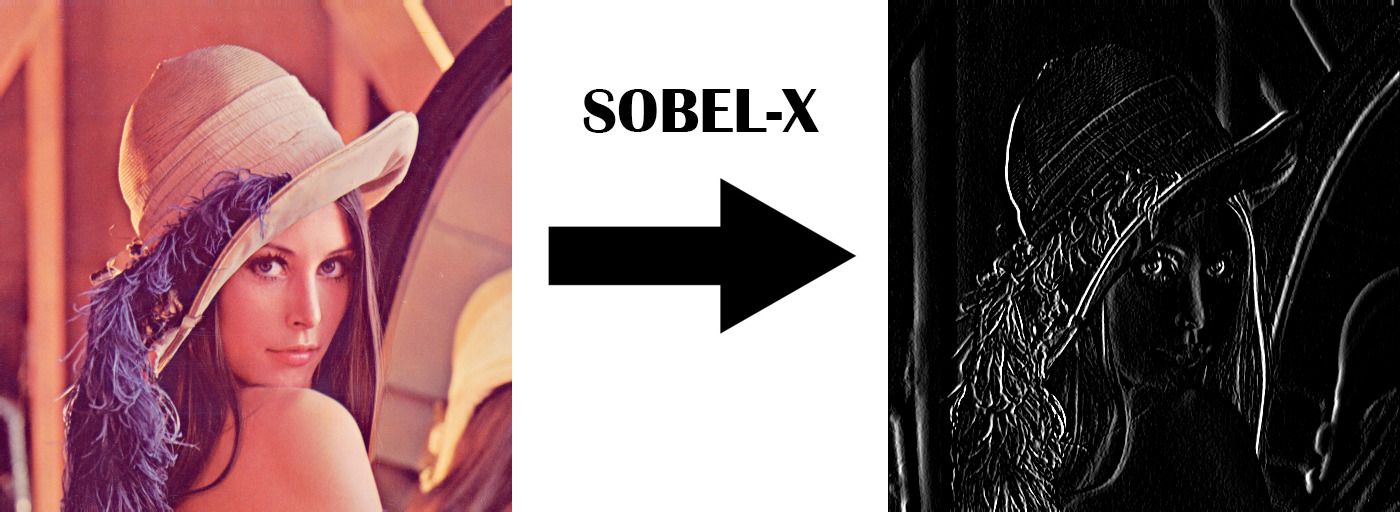
\includegraphics[width=\linewidth]{sobel-x}
	\caption{Esempio di Kernel Sobel-X}
\end{figure}
\begin{figure}[H]
	\centering
	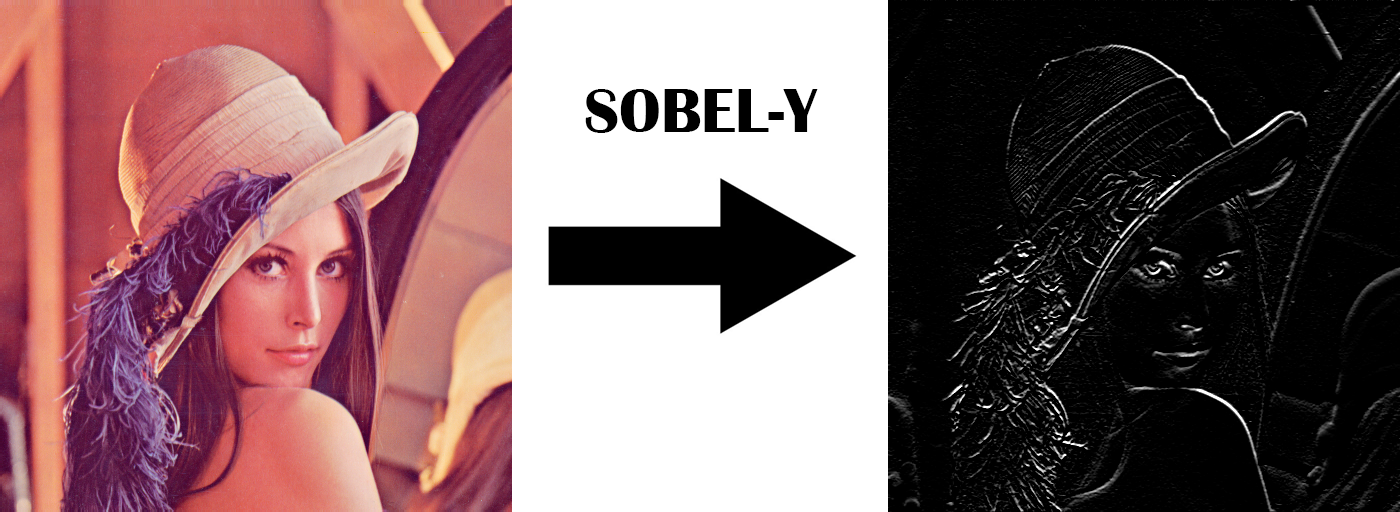
\includegraphics[width=\linewidth]{sobel-y}
	\caption{Esempio di Kernel Sobel-Y}
\end{figure}
\subsubsection{Prewitt-X e Prewitt-Y}
Simili ai kernel Sobel, i kernel di \textit{Prewitt-X} e \textit{Prewitt-Y} sono utilizzati per il rilevamento dei bordi. In particolare, \textit{Prewitt-X} evidenzia i cambiamenti di intensità orizzontali, mentre \textit{Prewitt-Y} quelli verticali.\newline
\begin{equation*}
	\text {Prewitt-X} = 
	\begin{bmatrix}
		-1 & 0 & 1 \\
		-1 & 0 & 1 \\
		-1 & 0 & 1
	\end{bmatrix},
	\quad
	\text {Prewitt-Y} = 
	\begin{bmatrix}
		-1 & -1 & -1 \\
		0 & 0 & 0 \\
		1 & 1 & 1
	\end{bmatrix},
\end{equation*}
\newline Quando vengono applicati a un'immagine tramite la convoluzione, calcolano le derivate parziali rispetto alle direzioni orizzontali e verticali, rispettivamente. Questo significa rilevano le variazioni di intensità lungo le linee orizzontali e verticali dell'immagine.

Rispetto ai kernel Sobel, producono un immanine meno nitida.
\begin{figure}[H]
	\centering
	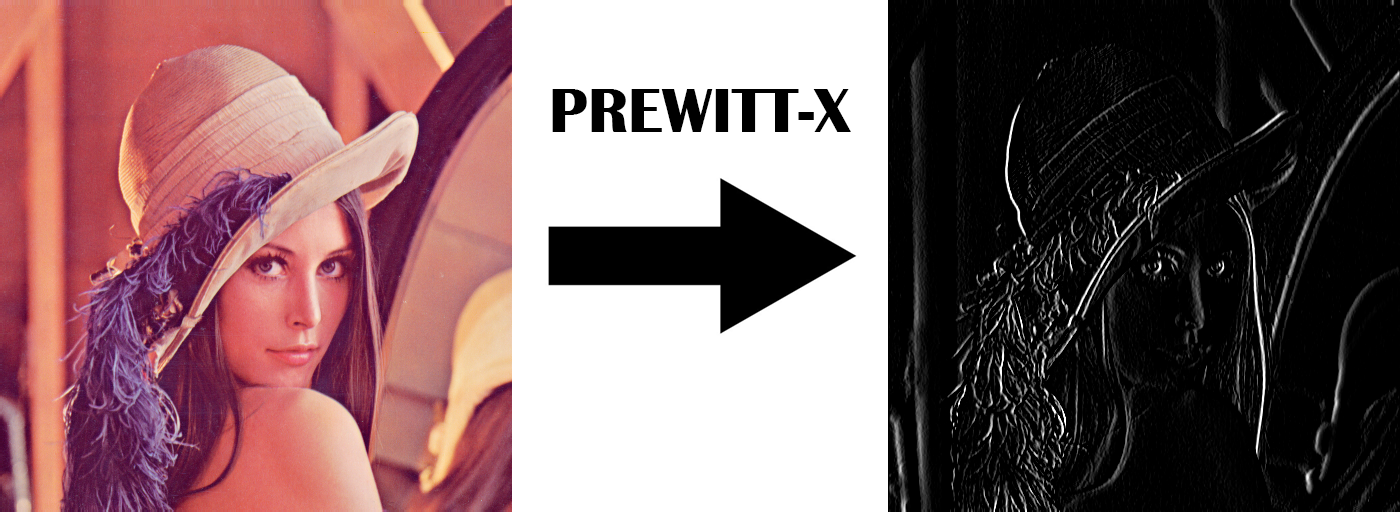
\includegraphics[width=\linewidth]{prewitt-x}
	\caption{Esempio di Kernel Prewitt-X}
\end{figure}
\begin{figure}[H]
	\centering
	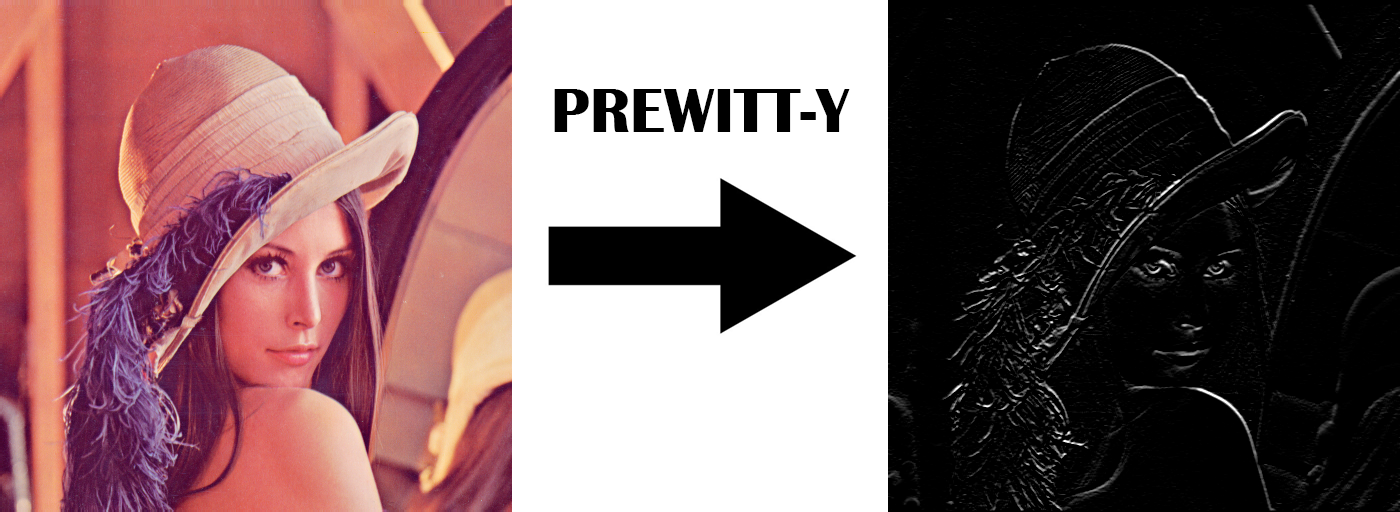
\includegraphics[width=\linewidth]{prewitt-y}
	\caption{Esempio di Kernel Prewitt-Y}
\end{figure}
\subsubsection{Laplacian}
Il kernel di \textit{Laplacian} è utilizzato per il rilevamento dei bordi o dei punti di discontinuità.\newline
\begin{equation*}
	\text {Laplacian} = 
	\begin{bmatrix}
		0 & -1 & 0 \\
		-1 & 4 & -1 \\
		0 & -1 & 0
	\end{bmatrix}
\end{equation*}
\newline Quando viene applicato a un'immagine tramite la convoluzione, produce una mappa dei gradienti del secondo ordine, che rappresenta la variazione dell'intensità dei pixel nell'immagine, generando un'immagine convoluta che evidenzia i bordi, le linee e altre caratteristiche forti dell'immagine.

Tuttavia, può anche produrre una risposta forte al rumore presente nell'immagine, poiché amplifica le variazioni di intensità in tutte le direzioni.
\begin{figure}[H]
	\centering
	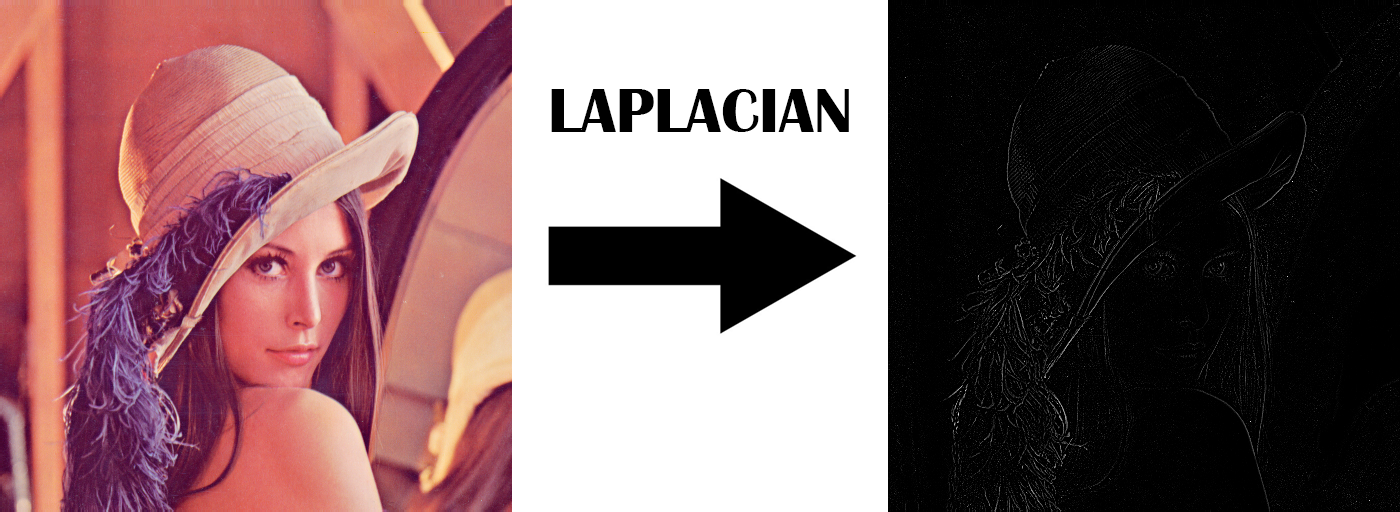
\includegraphics[width=\linewidth]{laplacian}
	\caption{Esempio di Kernel Laplacian}
\end{figure}
\subsubsection{Sharpen e High-Pass}
I kernel di \textit{Sharpen} e \textit{High-Pass} sono utilizzati per enfatizzare le componenti ad alta frequenza e attenuare quelle a bassa frequenza producendo un miglioramento dei dettagli di un'immagine.\newline
\begin{equation*}
	\text {Sharpen} = 
	\begin{bmatrix}
		0 & -1 & 0 \\
		-1 & 5 & -1 \\
		0 & -1 & 0
	\end{bmatrix},
	\quad
	\text {High-Pass} = 
	\begin{bmatrix}
		0 & -1/4 & 0 \\
		-1/4 & 2 & -1/4 \\
		0 & -1/4 & 0
	\end{bmatrix}
\end{equation*}
\newline Quando vengono applicati a un'immagine tramite la convoluzione, producono un'immagine convoluta in cui i bordi e i dettagli sono enfatizzati, migliorando il contrasto tra i pixel adiacenti e accentuando le transizioni di intensità.

Questo può portare ad un aspetto più definito e nitido dell'immagine.
\begin{figure}[H]
	\centering
	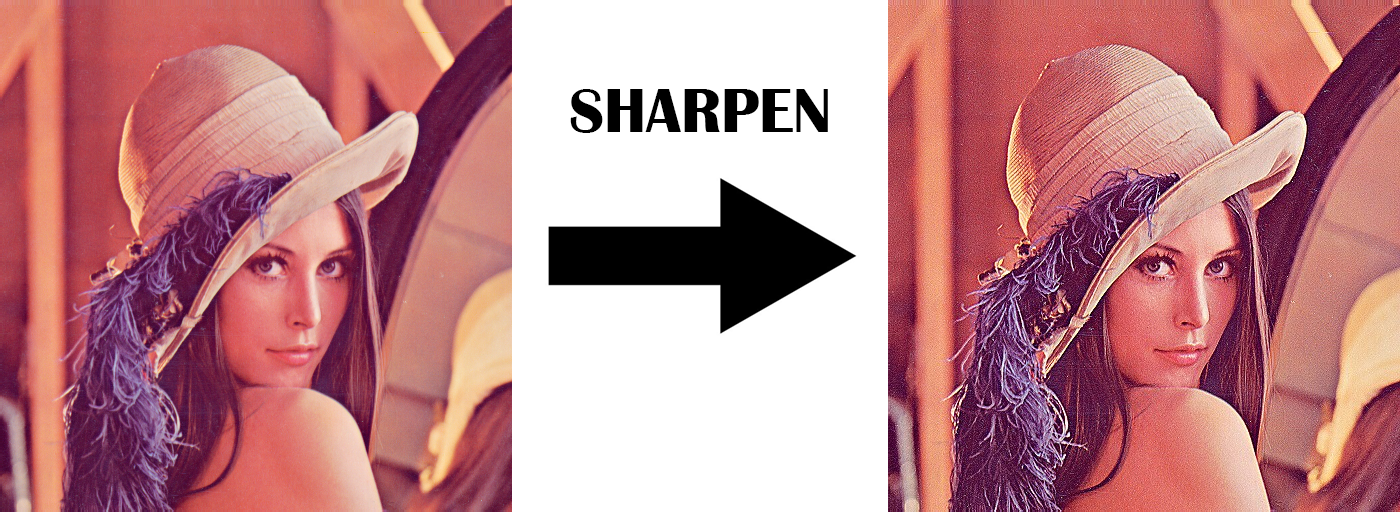
\includegraphics[width=\linewidth]{sharpen}
	\caption{Esempio di Kernel Sharpen}
\end{figure}
\begin{figure}[H]
	\centering
	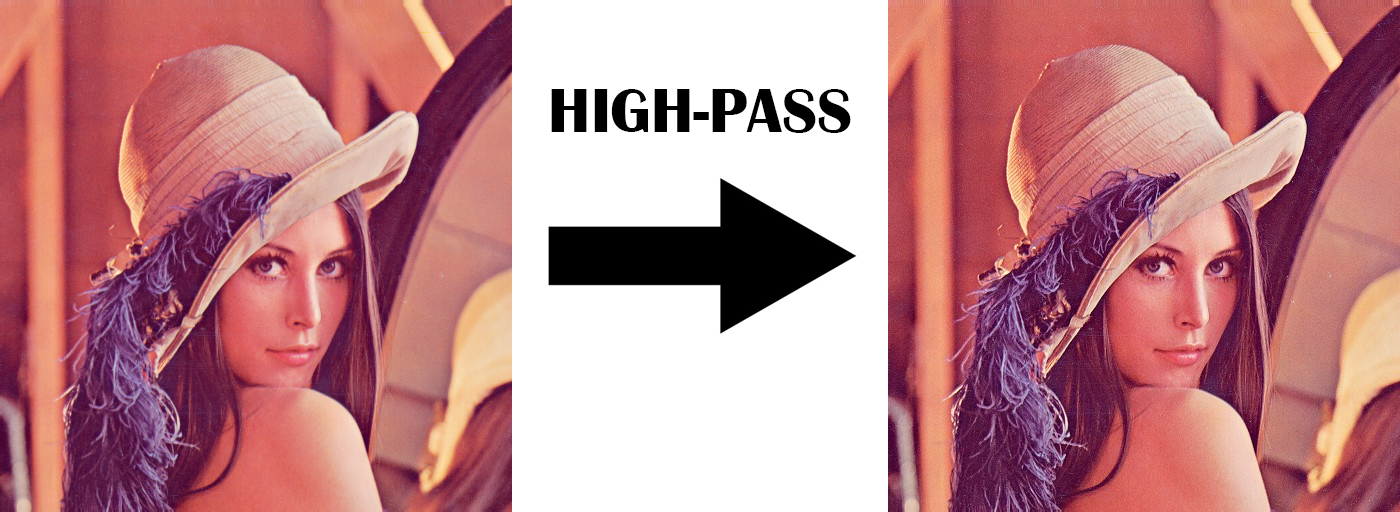
\includegraphics[width=\linewidth]{high-pass}
	\caption{Esempio di Kernel High-Pass}
\end{figure}
\subsubsection{Blur (Low-Pass)}
Il kernel di \textit{Low-Pass} è utilizzato per attenuare le componenti ad alta frequenza e mantiene le componenti a bassa frequenza, consentendo di eliminare il rumore e ottenere un'immagine più morbida.\newline
\begin{equation*}
	\text {Low-Pass} = 
	\begin{bmatrix}
		1/9 & 1/9 & 1/9 \\
		1/9 & 1/9 & 1/9 \\
		1/9 & 1/9 & 1/9
	\end{bmatrix}
\end{equation*}
\newline Quando viene applicato a un'immagine tramite la convoluzione, produce un'immagine convoluta in cui le transizioni brusche dell'intensità vengono attenuate e l'immagine risulta più sfocata.
\begin{figure}[H]
	\centering
	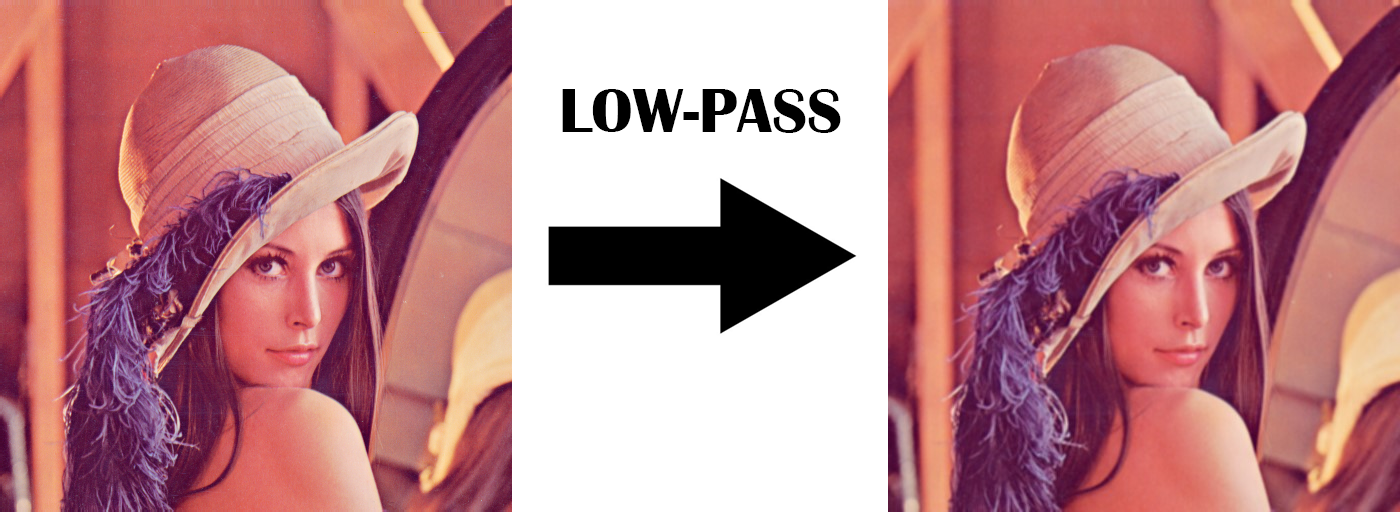
\includegraphics[width=\linewidth]{low-pass}
	\caption{Esempio di Kernel Low-Pass}
\end{figure}

\subsubsection{Blur (Gaussian)}
Il kernel di \textit{Gaussian} è utilizzato per eseguire una riduzione del rumore e una sfocatura dell'immagine\newline
\begin{equation*}
	\text {Gaussian 3x3} = 
	\begin{bmatrix}
		1/16 & 2/16 & 1/16 \\
		2/16 & 4/16 & 2/16 \\
		1/16 & 2/16 & 1/16
	\end{bmatrix}
\end{equation*}
\newline Quando viene applicato a un'immagine tramite la convoluzione, produce un effetto di sfocatura, riducendo le variazioni di intensità tra i pixel e attenuando il rumore ad alta frequenza.

L'uso del kernel gaussiano permette di ottenere una sfocatura più naturale e graduale rispetto ad altri filtri di sfocatura più semplici, poiché tiene conto delle distribuzioni di intensità circostanti, rendendo la transizione da un pixel all'altro più morbida e realistica.

Fornendo una dimensione e un valore sigma, Benchmarker può generare un kernel di Gaussian che rispetti i parametri forniti.

La logica per la generazione di un kernel gaussiano di una certa \textit{dimensione} con un certo \textit{sigma} implementata in Python è presente in appendice: \ref{appendix:gauss}
\begin{figure}[H]
	\centering
	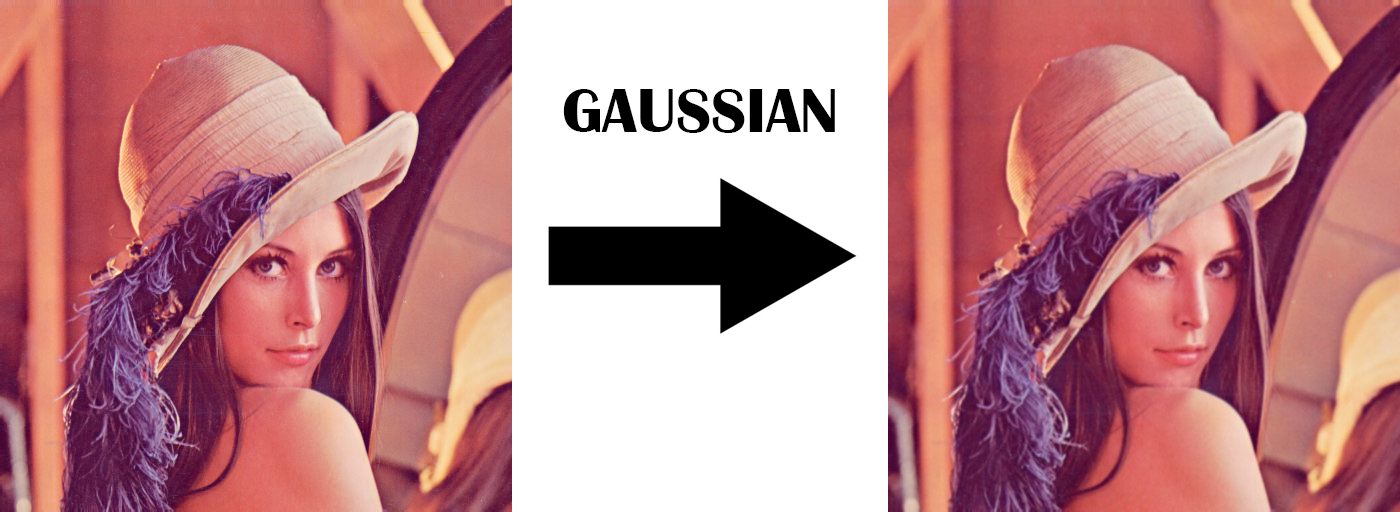
\includegraphics[width=\linewidth]{gaussian}
	\caption{Esempio di Kernel Gaussian}
\end{figure}

\subsection{Operatori Morfologici}
Gli \textit{operatori morfologici} sono utilizzati per manipolare la forma, la struttura e le caratteristiche di un'immagine. Queste operazioni si basano su principi matematici che coinvolgono l'interazione tra un \textit{elemento strutturante} e i pixel dell'immagine.

Gli \textit{elementi strutturanti}, anche chiamati \textit{kernel di forma}, sono matrici che definiscono la forma e la dimensione dell'area circostante a ciascun pixel durante l'applicazione degli operatori morfologici. \textit{Questi elementi strutturanti svolgono un ruolo cruciale nel determinare l'effetto dell'operazione morfologica sull'immagine}.\newline\newline
\noindent\textit{Benchmarker} implementa e permette la selezione dei seguenti elementi strutturali:
\begin{equation*}
	\text {Square} = 
	\begin{bmatrix}
		1 & 1 & 1\\
		1 & 1 & 1\\
		1 & 1 & 1
	\end{bmatrix}
	\text {Cross} = 
	\begin{bmatrix}
		0 & 1 & 0\\
		1 & 1 & 1\\
		0 & 1 & 0
	\end{bmatrix}
	\text {Line} = 
	\begin{bmatrix}
		0 & 0 & 0\\
		1 & 1 & 1\\
		0 & 0 & 0
	\end{bmatrix}
	\text {Circle} = 
	\begin{bmatrix}
		0 & 1 & 1 & 1 & 0\\
		1 & 1 & 1 & 1 & 1\\
		1 & 1 & 1 & 1 & 1\\
		1 & 1 & 1 & 1 & 1\\
		0 & 1 & 1 & 1 & 0
	\end{bmatrix}
\end{equation*}

\noindent \textit{Benchmarker} implementa gli operatori morfologici di erosione e dilatazione, i cui codici sono presenti in appendice: \ref{appendix:erosion}.

\subsubsection{Erosione}
L'erosione è un'operazione morfologica che riduce le regioni o i dettagli di un'immagine. Durante l'erosione, ogni pixel nell'immagine viene confrontato con il corrispondente sotto l'elemento strutturante. Se tutti i pixel sottostanti l'elemento strutturante sono \textit{attivi}, cioè hanno un valore di intensità alto, il pixel corrispondente nell'immagine risultante viene mantenuto attivo. In caso contrario, il pixel viene disattivato o eliminato. L'erosione tende a ridurre la dimensione degli oggetti e a rimuovere piccoli dettagli, consentendo di separare le regioni connesse.

\begin{figure}[H]
	\centering
	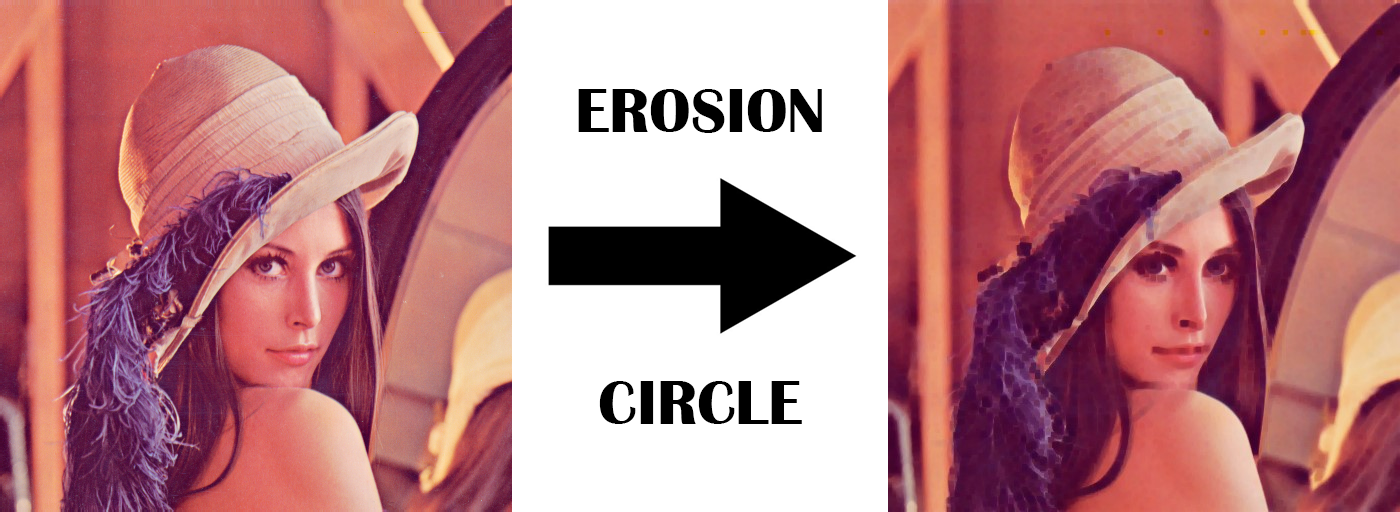
\includegraphics[width=\linewidth]{erosion}
	\caption{Esempio Erosione con elemento strutturante Circle}
\end{figure}

\subsubsection{Dilatazione}
La dilatazione è un'altra operazione morfologica che ha l'effetto opposto dell'erosione. Durante la dilatazione, ogni pixel nell'immagine viene confrontato con il corrispondente sotto l'elemento strutturante. Se almeno un pixel sottostante l'elemento strutturante è \textit{attivo}, il pixel corrispondente nell'immagine risultante viene attivato o mantenuto attivo. La dilatazione tende ad espandere le regioni e a unire gli oggetti vicini.


\begin{figure}[H]
	\centering
	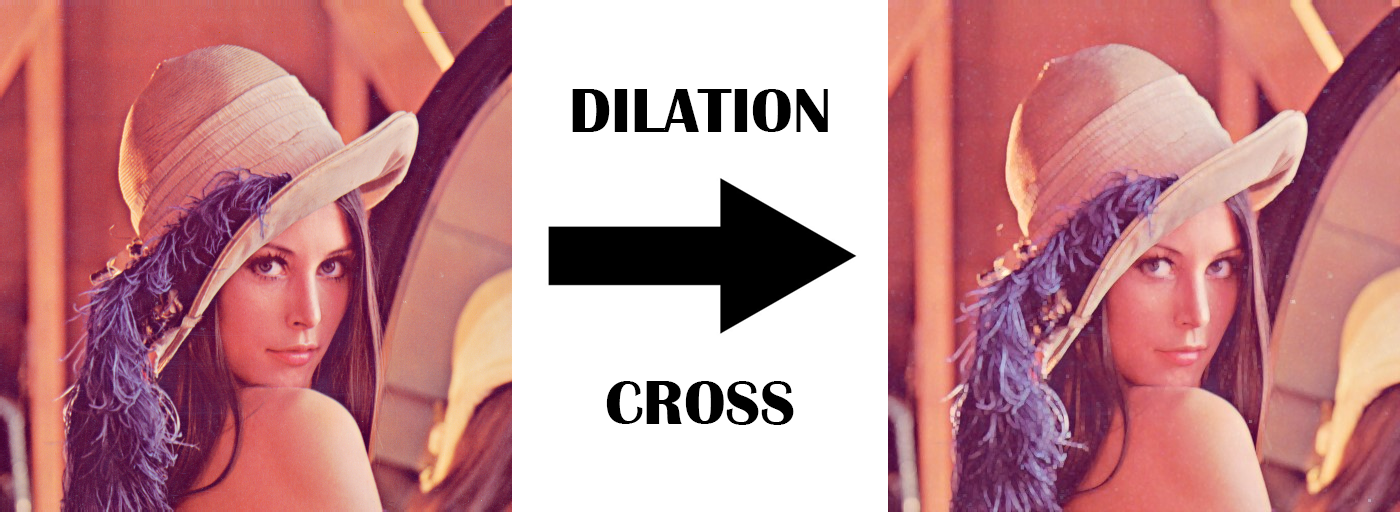
\includegraphics[width=\linewidth]{dilation}
	\caption{Esempio Dilatazione con elemento strutturante Cross}
\end{figure}

\subsection{Filtri di Noise Reduction}
I filtri di \textit{noise reduction}, o \textit{filtri di riduzione del rumore}, sono utilizzati per mitigare o eliminare il rumore presente nelle immagini digitali. Il rumore può essere causato da vari fattori, come le imperfezioni del sensore, le interferenze elettriche o il processo di acquisizione dell'immagine.

L'obiettivo principale è quello di migliorare la qualità dell'immagine, rimuovendo o riducendo il rumore senza influire eccessivamente sulla nitidezza e sui dettagli importanti dell'immagine.

\textit{Benchmarker} implementa il \textit{mean filter} e il \textit{bilateral} filter, , i cui codici sono presenti in appendice: \ref{appendix:mean}.

\subsubsection{Mean Filter}
Il \textit{filtro di media}, detto anche \textit{mean filter}, è uno dei filtri di noise reduction più semplici ed efficaci. Sostituisce il valore di ciascun pixel nell'immagine con la media dei valori dei pixel nell'intorno del pixel stesso.

In pratica, il filtro di media calcola la media aritmetica dei valori dei pixel all'interno di una finestra quadrata e sostituisce il valore del pixel corrente con questa media.

Questo processo aiuta a ridurre il rumore, poiché il rumore casuale tende ad avere un effetto minore sulla media dei valori dei pixel.

La dimensione dell'intorno viene decisa dall'utente al momento della selezione del filtro di media.

\begin{figure}[H]
	\centering
	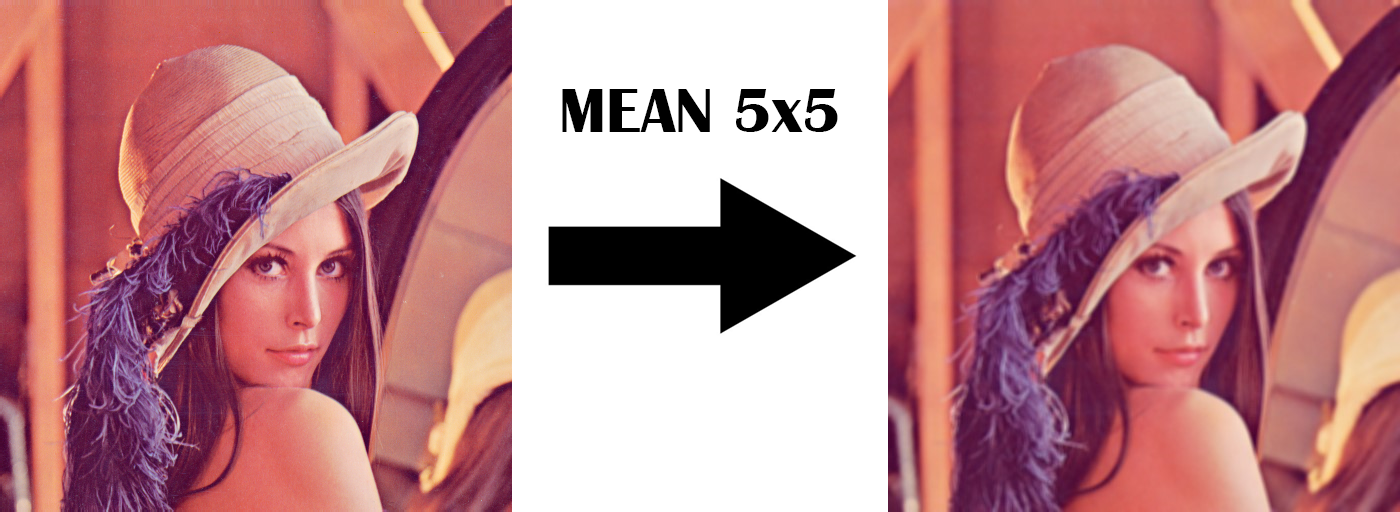
\includegraphics[width=\linewidth]{mean}
	\caption{Esempio di filtro di media 5x5}
\end{figure}

\subsubsection{Bilateral Filter}
Il \textit{filtro bilaterale}, detto anche \textit{bilateral filter} offre una maggiore flessibilità nel mantenere i confini e i dettagli dell'immagine. 

A differenza del filtro di media, il filtro bilaterale considera non solo i valori dei pixel nell'intorno, ma anche le differenze di intensità tra i pixel.

Questo filtro calcola una media ponderata dei valori dei pixel all'interno di una finestra, in base alla distanza spaziale tra i pixel e alla differenza di intensità tra i pixel.

Ciò significa che i pixel che sono simili in termini di intensità e vicini spazialmente avranno un peso maggiore nella media ponderata, mentre i pixel con differenze significative di intensità avranno un peso minore. In questo modo, il filtro bilaterale può ridurre il rumore, preservando al contempo i dettagli e i confini dell'immagine.

La dimensione dell'intorno, distanza spaziale e la differenza d'intensità vengono decisi dall'utente al momento della selezione del filtro bilaterale.

\begin{figure}[H]
	\centering
	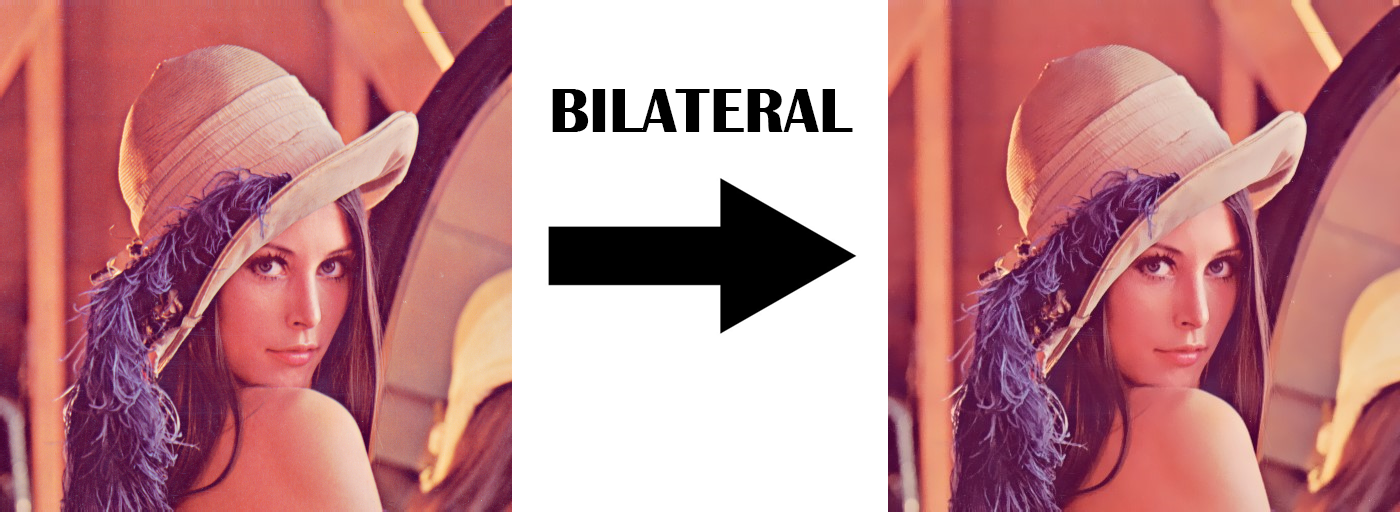
\includegraphics[width=\linewidth]{bilateral}
	\caption{Esempio di filtro bilaterale}
\end{figure}

\subsection{Canny}
Il \textit{filtro di Canny}, chiamato anche \textit{algoritmo di Canny}, è un popolare filtro di \textit{edge detection}. È un algoritmo composto da più passaggi che combinati insieme forniscono una buona precisione nel rilevamento dei bordi, riducendo al contempo il rumore.

L'algoritmo di Canny opera secondo i seguenti passaggi:
\begin{itemize}
	\item \textit{Riduzione del rumore}: l'immagine di input viene filtrata per ridurre il rumore. Viene applico un filtro di \textit{smoothing}, come ad esempio il \textit{filtro di Gaussian} per quanto riguarda Benchmarker, per sfocare leggermente l'immagine e ridurre il rumore indesiderato;
	
	\item \textit{Calcolo del gradiente}: viene \textit{calcolato il gradiente} dell'immagine utilizzando\textit{ operatori di differenza di intensità}, come ad esempio il filtro di Sobel. Il gradiente rappresenta la variazione di intensità dei pixel nell'immagine e fornisce informazioni sulla direzione e l'intensità dei cambiamenti di intensità;
	
	\item \textit{Suppressione dei non-maxima}: viene eseguita una soppressione dei non-maxima per sottolineare solo i punti di massima intensità lungo i bordi rilevati. Questo passaggio aiuta a sottolineare i bordi sottili mantenendo solo i punti di massima intensità lungo le direzioni dei gradienti;
	
	\item \textit{Linking dei bordi}: viene applicata una tecnica chiamata \textit{isteresi} per collegare i bordi rimanenti. Questo passaggio coinvolge l'impostazione di due soglie, una soglia inferiore e una soglia superiore. I pixel con intensità superiore alla soglia superiore vengono considerati come \textit{bordi forti}, mentre i pixel con intensità tra la soglia inferiore e la soglia superiore vengono considerati come \textit{bordi deboli}. I bordi deboli vengono mantenuti solo se sono collegati a bordi forti. In questo modo, si cerca di conservare solo i bordi rilevanti e ridurre l'inclusione di rumore;
\end{itemize}
\noindent Il risultato finale dell'algoritmo di Canny è un'\textit{immagine binaria} che rappresenta i bordi individuati nell'immagine di input. I bordi sono rappresentati come linee sottili che corrispondono ai confini tra regioni di intensità diversa.

La \textit{dimensione del kernel} e il valore \textit{sigma} del filtro di Gaussian e la \textit{soglie inferiore e superiore} vengono decisi dall'utente al momento della selezione del filtro di Canny. \newline\newline
\noindent La logica implementativa di Canny è presente in appendice: \ref{appendix:canny}.
\begin{figure}[H]
	\centering
	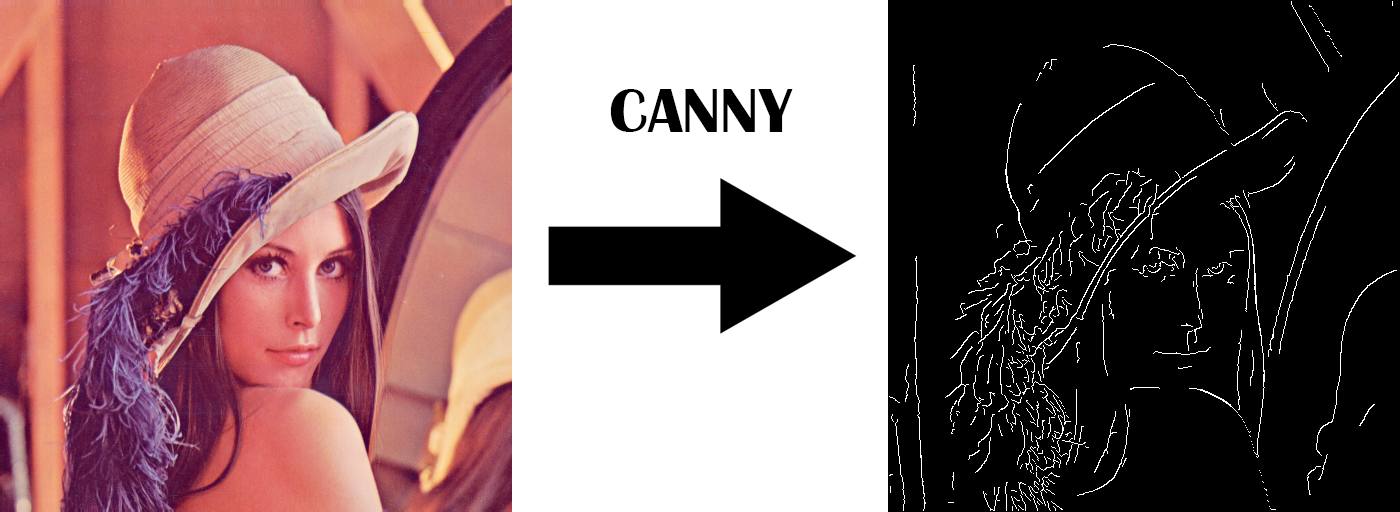
\includegraphics[width=\linewidth]{canny}
	\caption{Esempio di Canny Edge Detection}
\end{figure}